\section{Figures}\label{sec:figures}

\begin{figure}[H]
    \centering
    \begin{subfigure}{.32\textwidth}
        \centering
        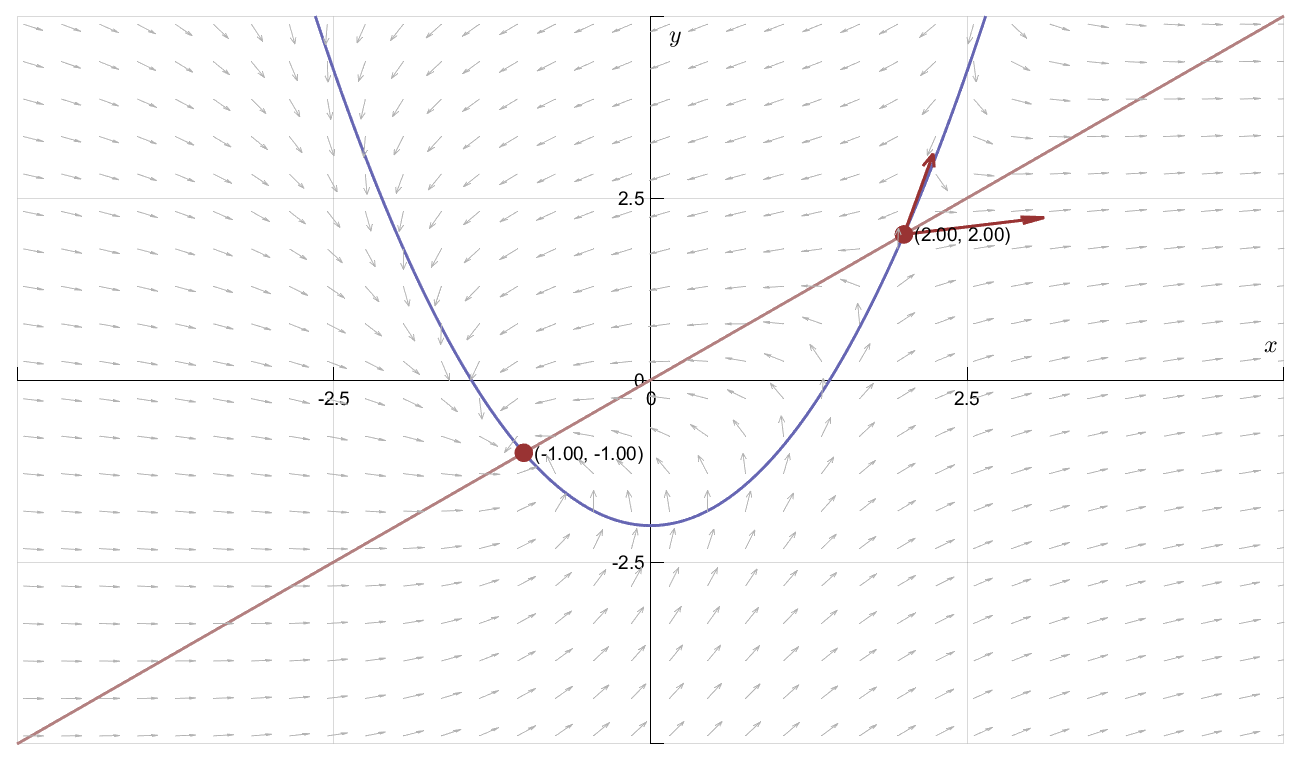
\includegraphics[width=\textwidth]{fig2.1_a.png}
        \caption{$\alpha=-2$}
    \end{subfigure}
    \begin{subfigure}{.32\textwidth}
        \centering
        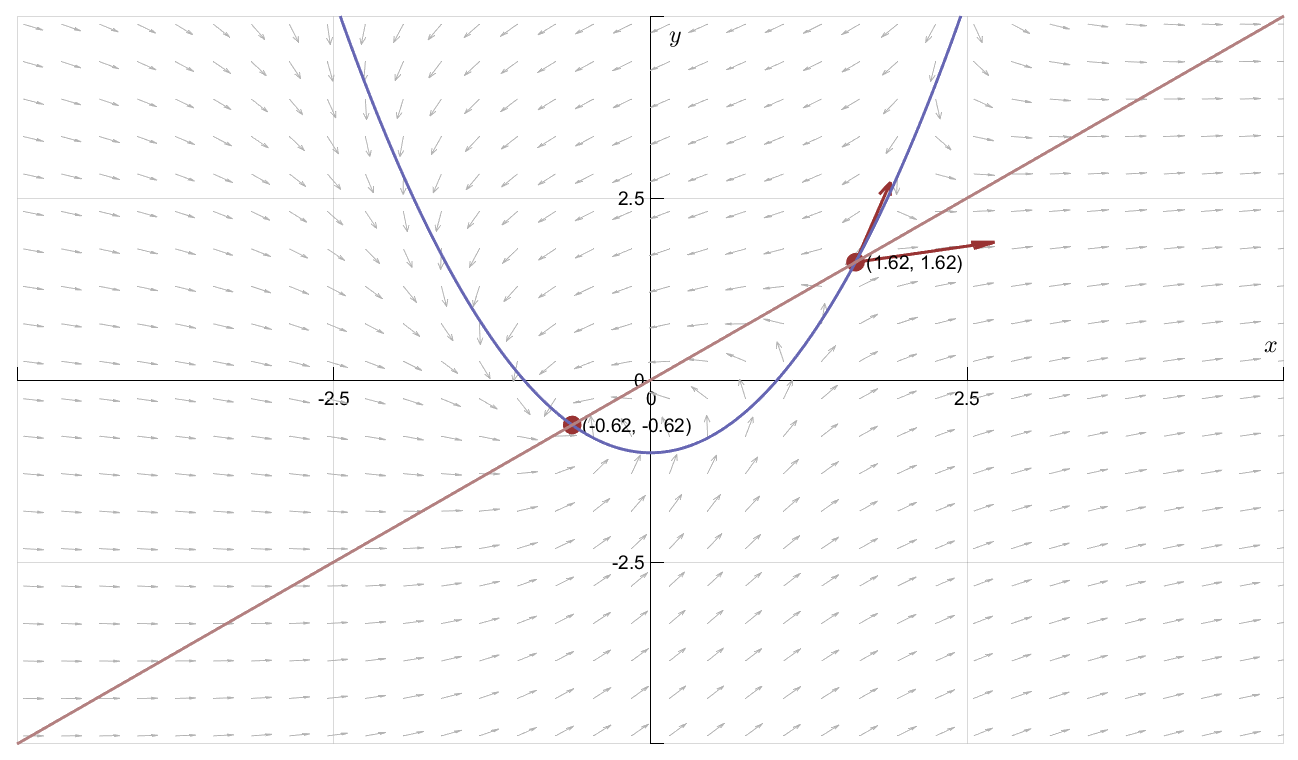
\includegraphics[width=\textwidth]{fig2.1_b.png}
        \caption{$\alpha=-1$}
    \end{subfigure}
    \begin{subfigure}{.32\textwidth}
        \centering
        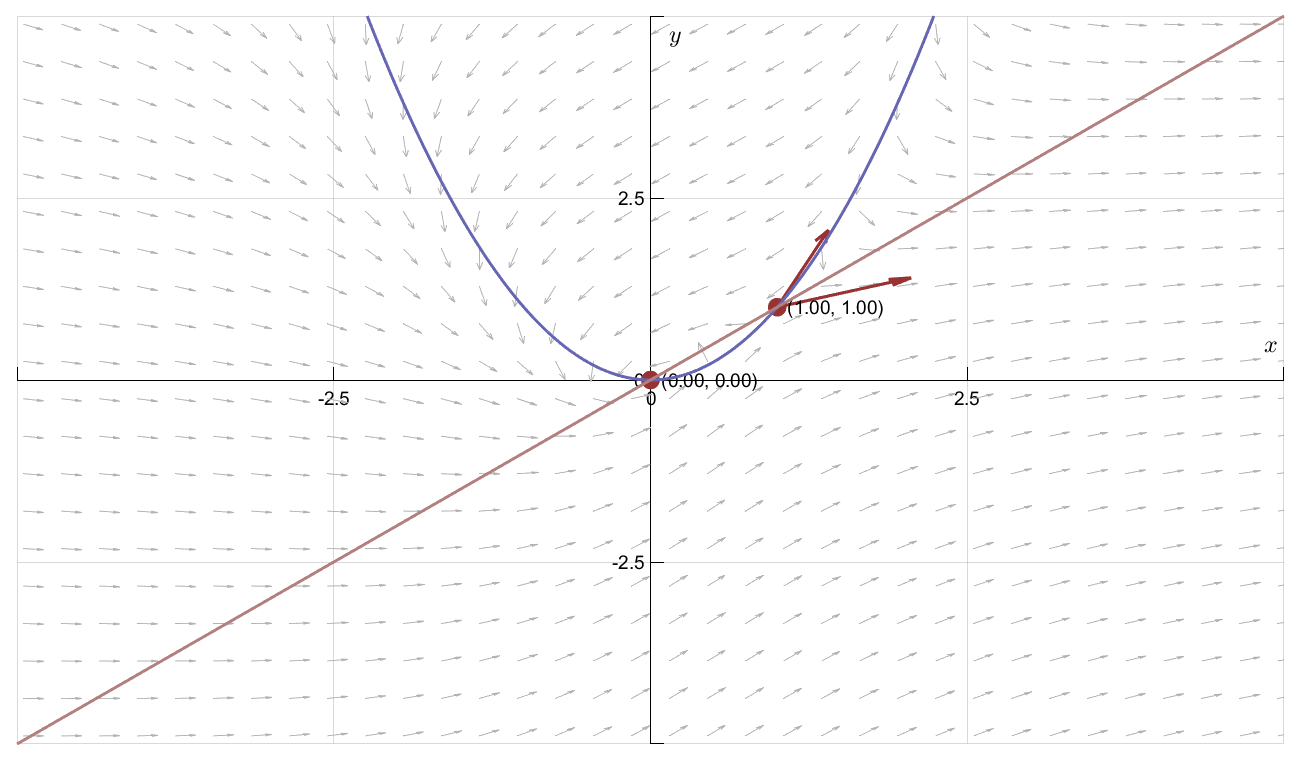
\includegraphics[width=\textwidth]{fig2.1_c.png}
        \caption{$\alpha=0$}
    \end{subfigure}
    \begin{subfigure}{.49\textwidth}
        \centering
        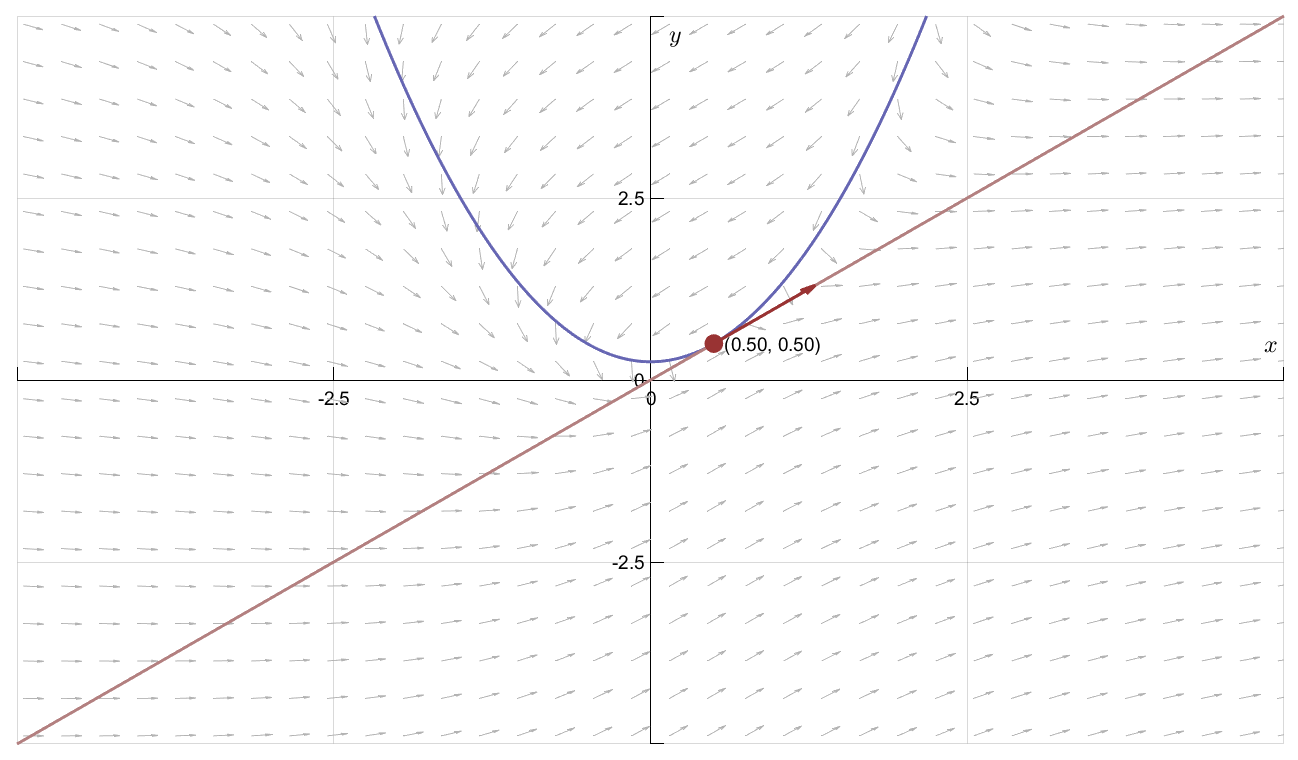
\includegraphics[width=\textwidth]{fig2.1_d.png}
        \caption{$\alpha=1/4$}
    \end{subfigure}
    \begin{subfigure}{.49\textwidth}
        \centering
        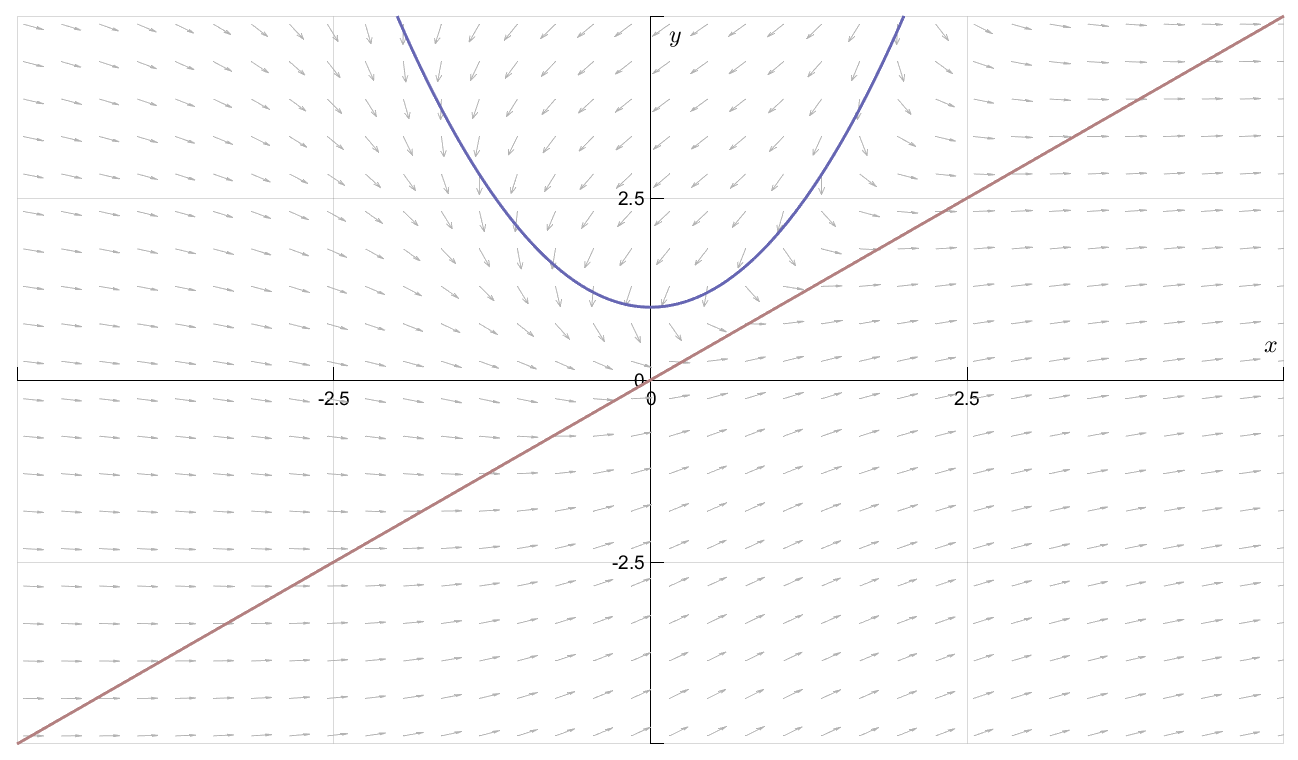
\includegraphics[width=\textwidth]{fig2.1_e.png}
        \caption{$\alpha=1$}
    \end{subfigure}
    \caption{Nullcline Analysis for potential system 1}
    \label{fig:1}
\end{figure}

\begin{figure}[H]
    \centering
    \begin{subfigure}{.32\textwidth}
        \centering
        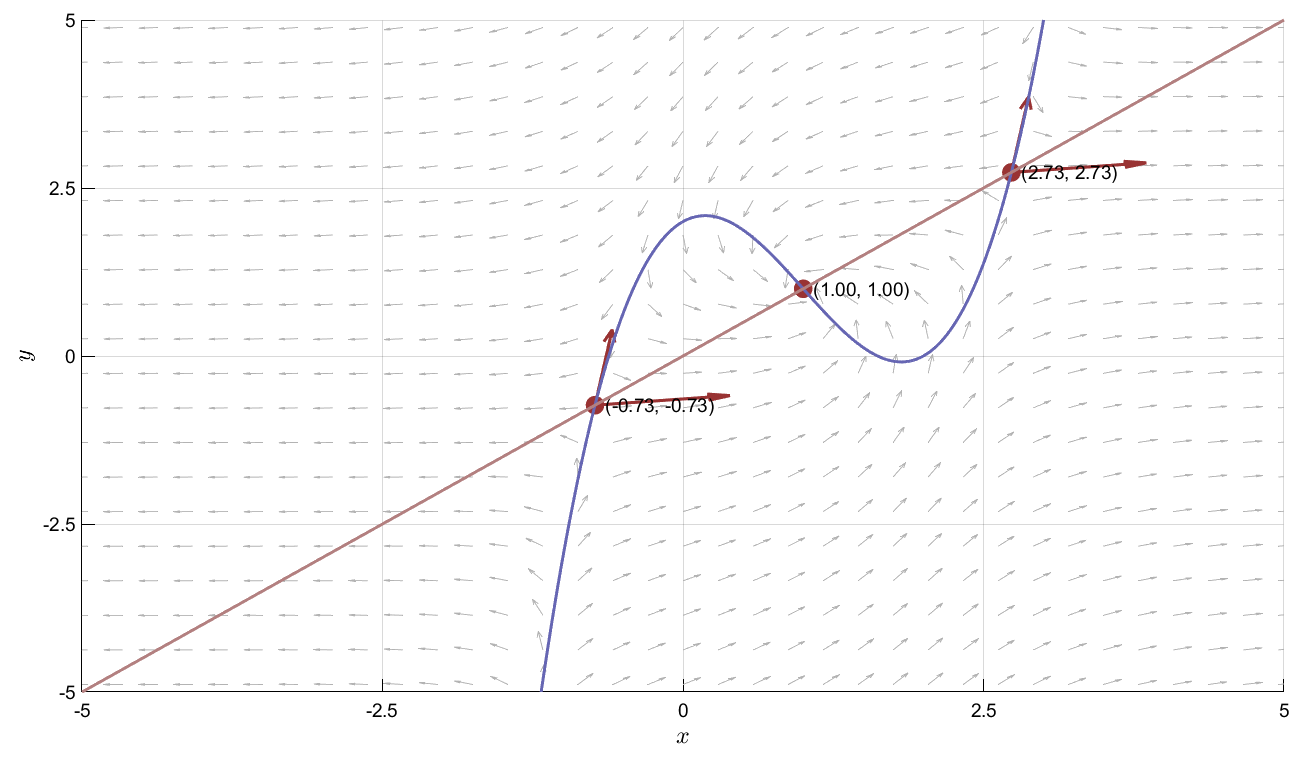
\includegraphics[width=\textwidth]{fig2.2_a.png}
        \caption{$\beta=-2$}
    \end{subfigure}
    \begin{subfigure}{.32\textwidth}
        \centering
        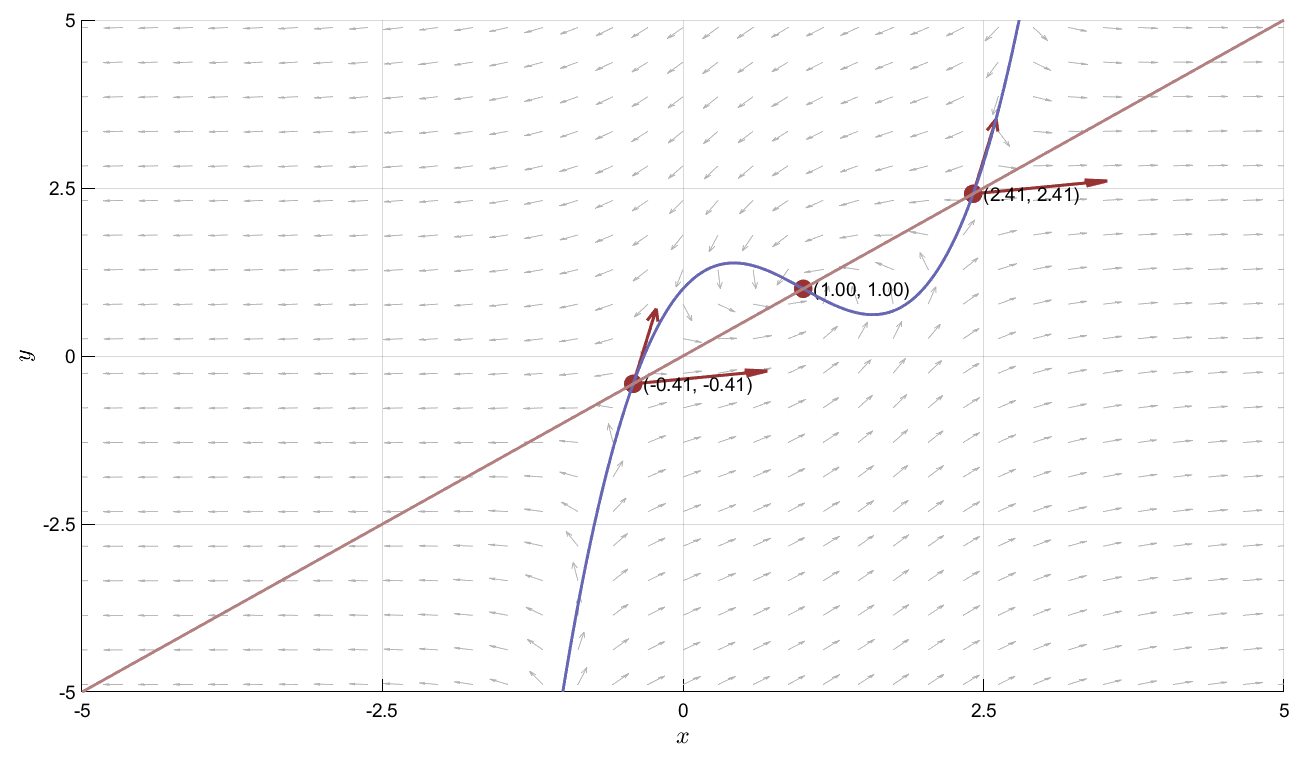
\includegraphics[width=\textwidth]{fig2.2_b.png}
        \caption{$\beta=-1$}
    \end{subfigure}
    \begin{subfigure}{.32\textwidth}
        \centering
        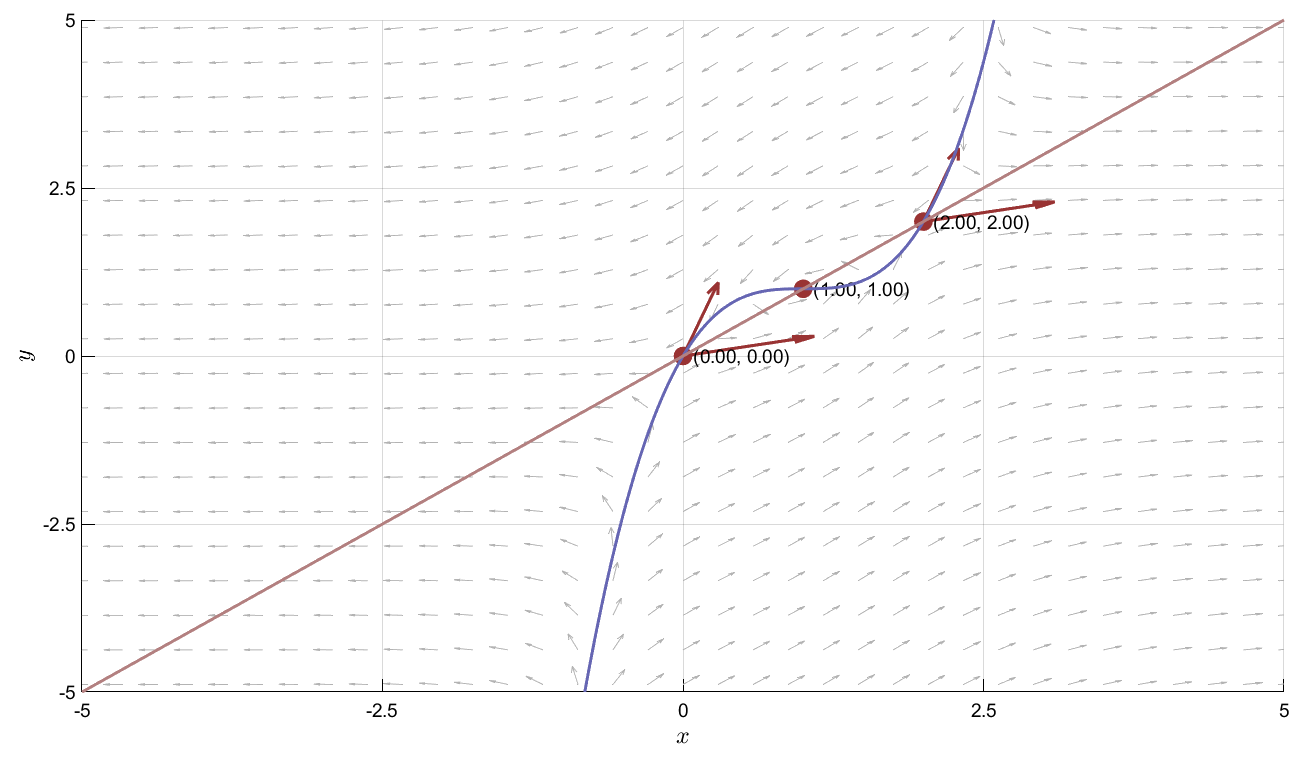
\includegraphics[width=\textwidth]{fig2.2_c.png}
        \caption{$\beta=0$}
    \end{subfigure}
    \begin{subfigure}{.49\textwidth}
        \centering
        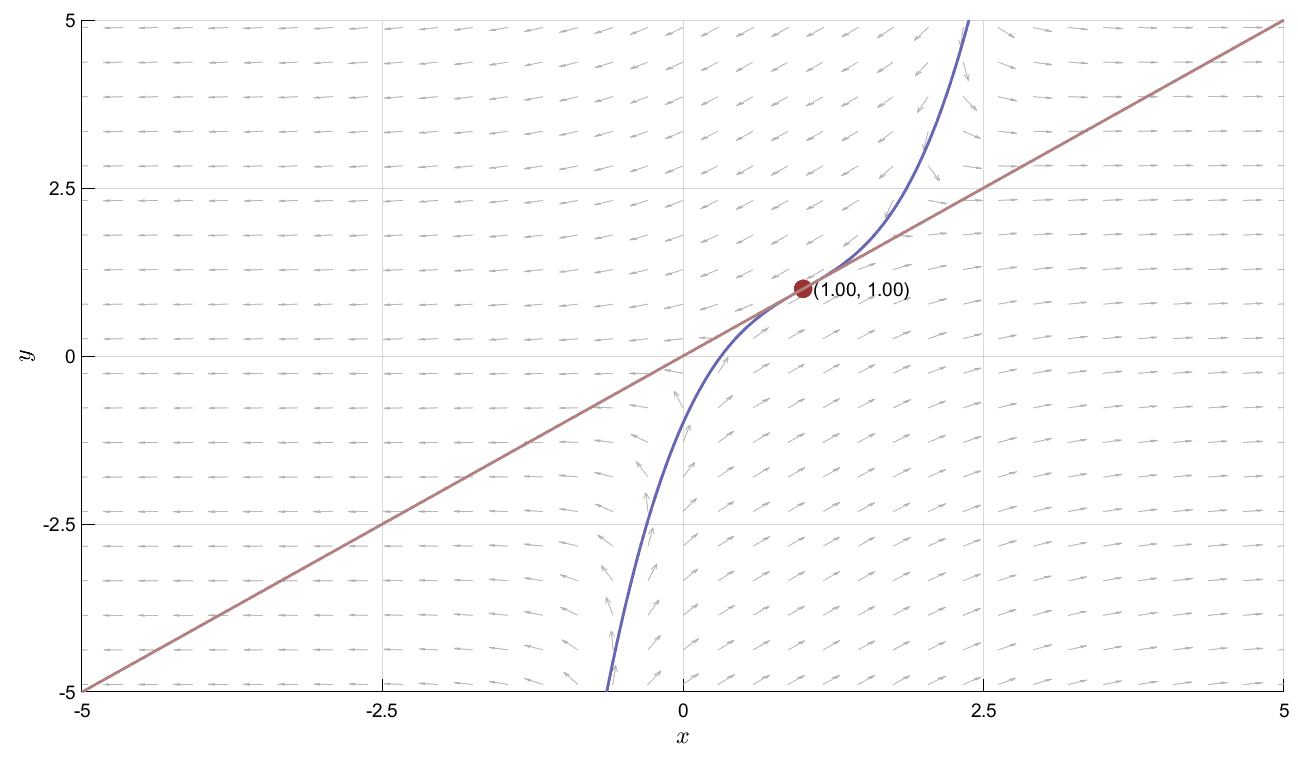
\includegraphics[width=\textwidth]{fig2.2_d.png}
        \caption{$\beta=1$}
    \end{subfigure}
    \begin{subfigure}{.49\textwidth}
        \centering
        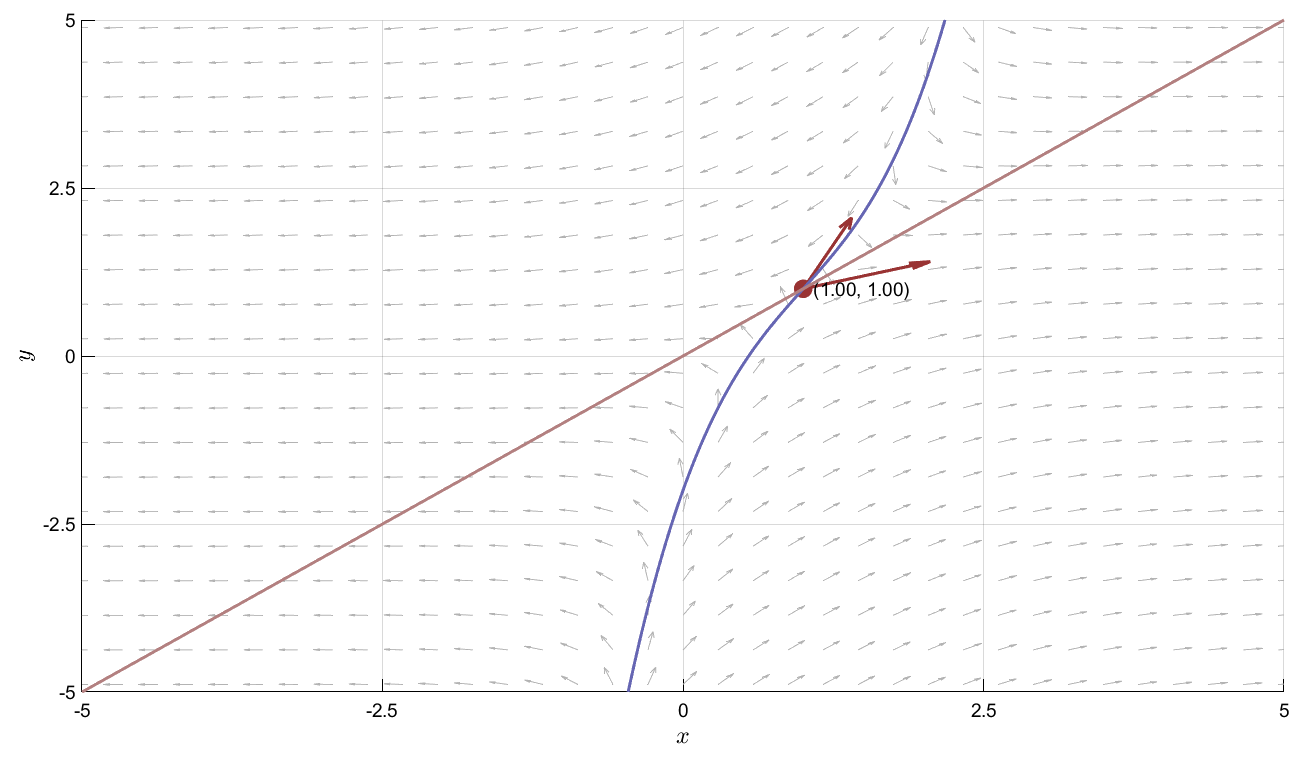
\includegraphics[width=\textwidth]{fig2.2_e.png}
        \caption{$\beta=2$}
    \end{subfigure}
    \caption{Nullcline Analysis for potential system 2}
    \label{fig:2}
\end{figure}

\begin{figure}[H]
    \centering
    \begin{subfigure}{.32\textwidth}
        \centering
        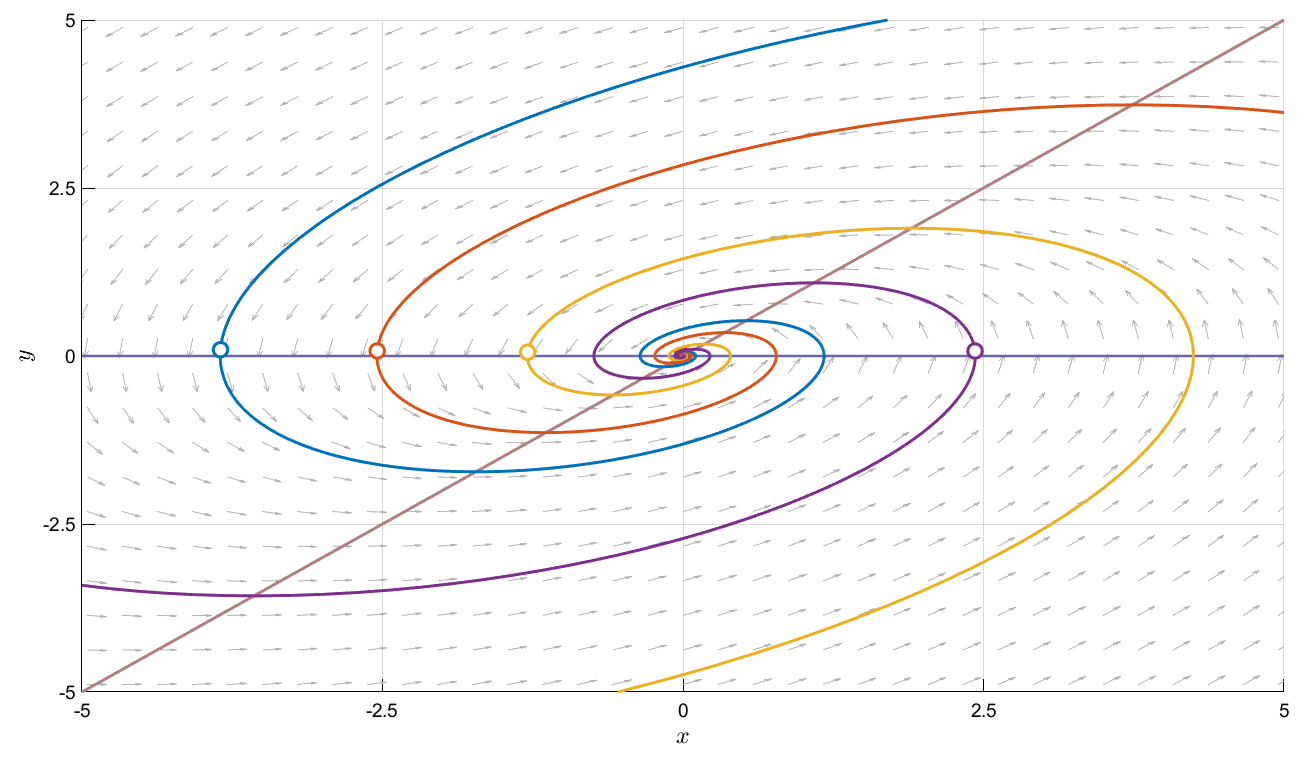
\includegraphics[width=\textwidth]{fig2.3_a.png}
        \caption{$\gamma=-1$}
    \end{subfigure}
    \begin{subfigure}{.32\textwidth}
        \centering
        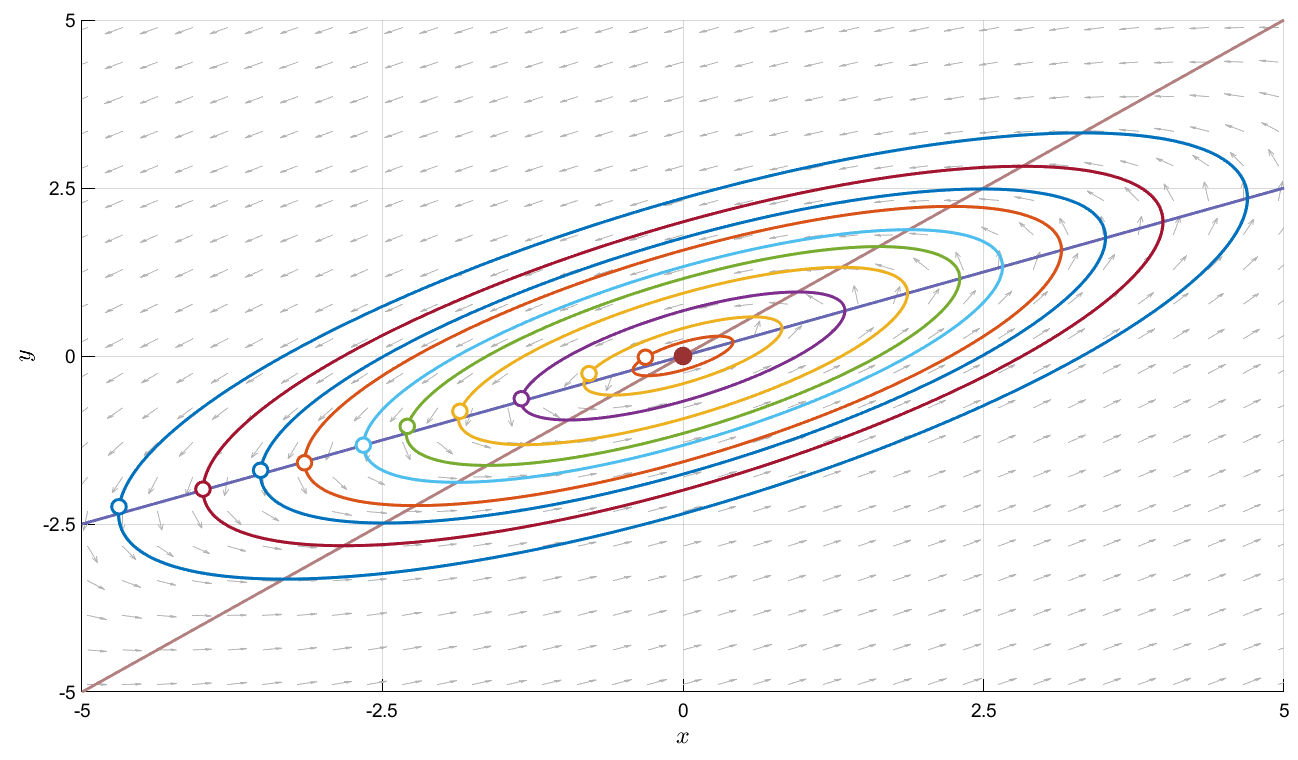
\includegraphics[width=\textwidth]{fig2.3_b.png}
        \caption{$\gamma=0$}
    \end{subfigure}
    \begin{subfigure}{.32\textwidth}
        \centering
        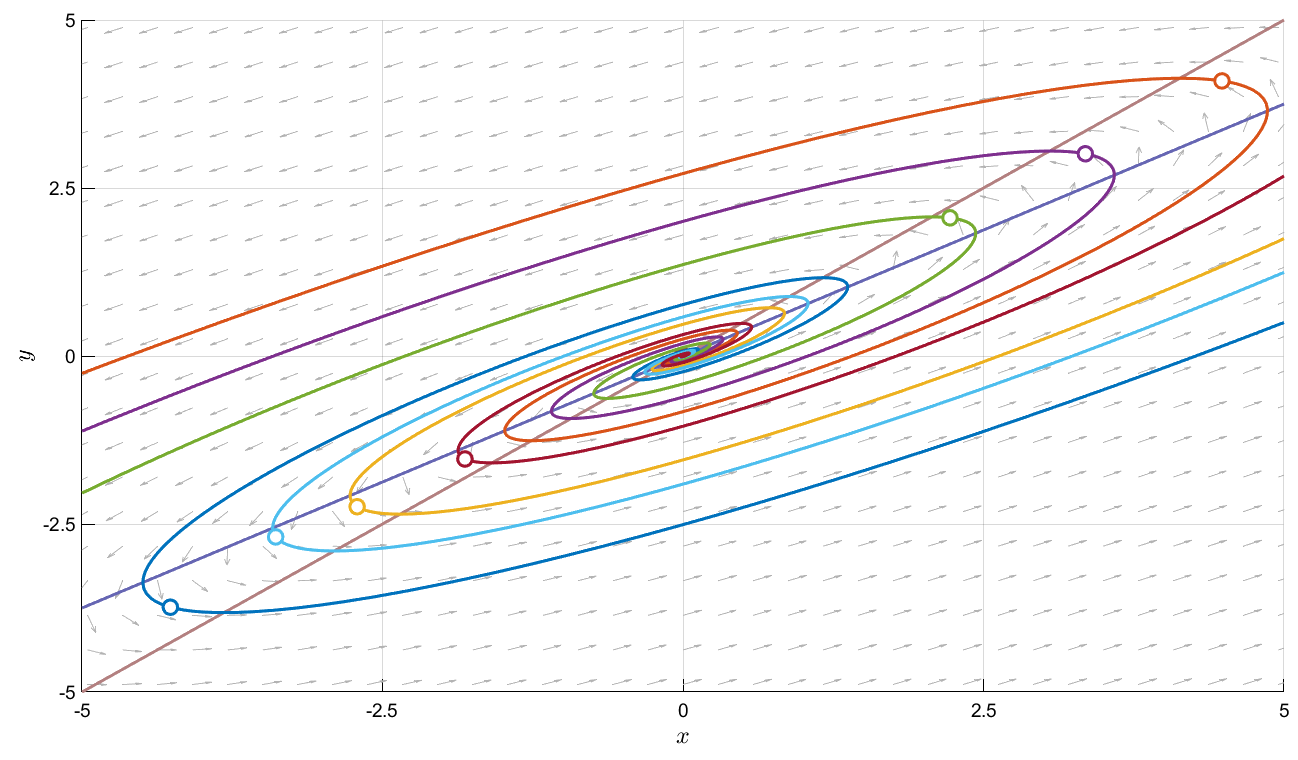
\includegraphics[width=\textwidth]{fig2.3_c.png}
        \caption{$\gamma=1/2$}
    \end{subfigure}
    \begin{subfigure}{.49\textwidth}
        \centering
        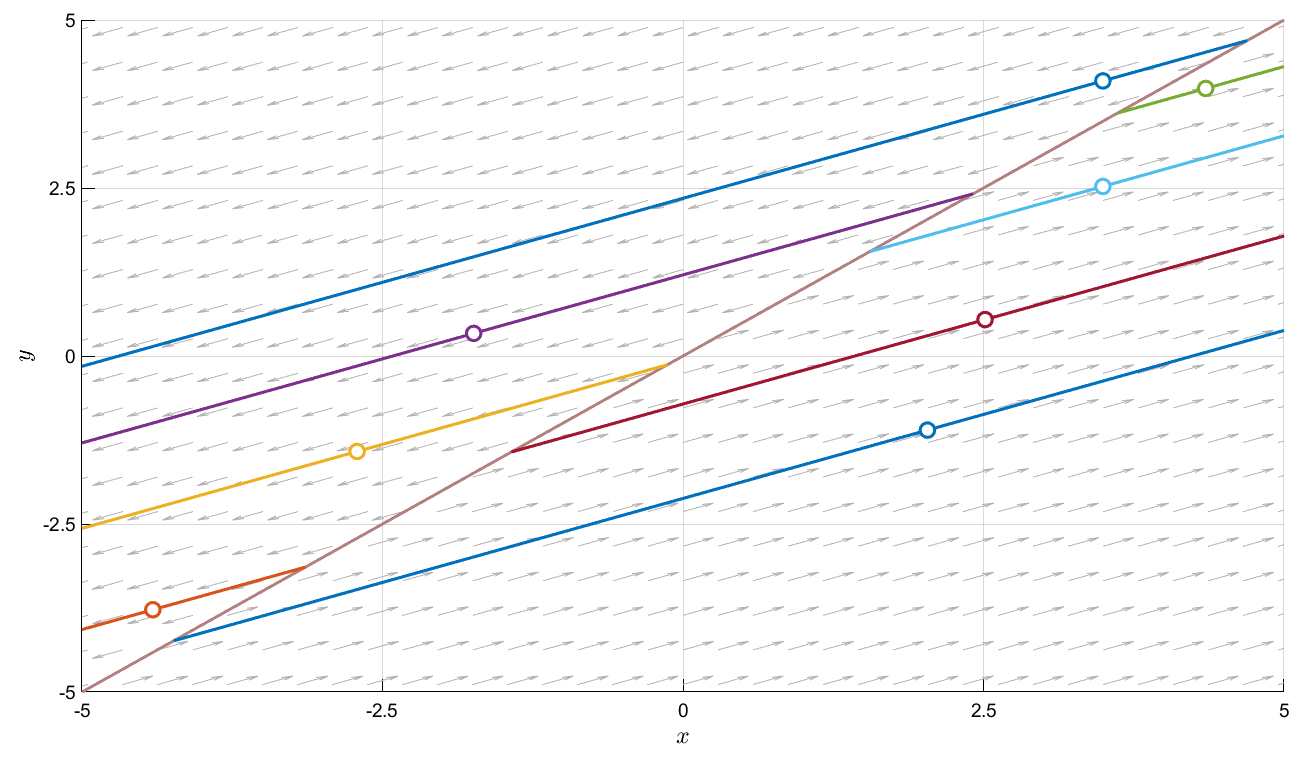
\includegraphics[width=\textwidth]{fig2.3_d.png}
        \caption{$\gamma=1$}
    \end{subfigure}
    \begin{subfigure}{.49\textwidth}
        \centering
        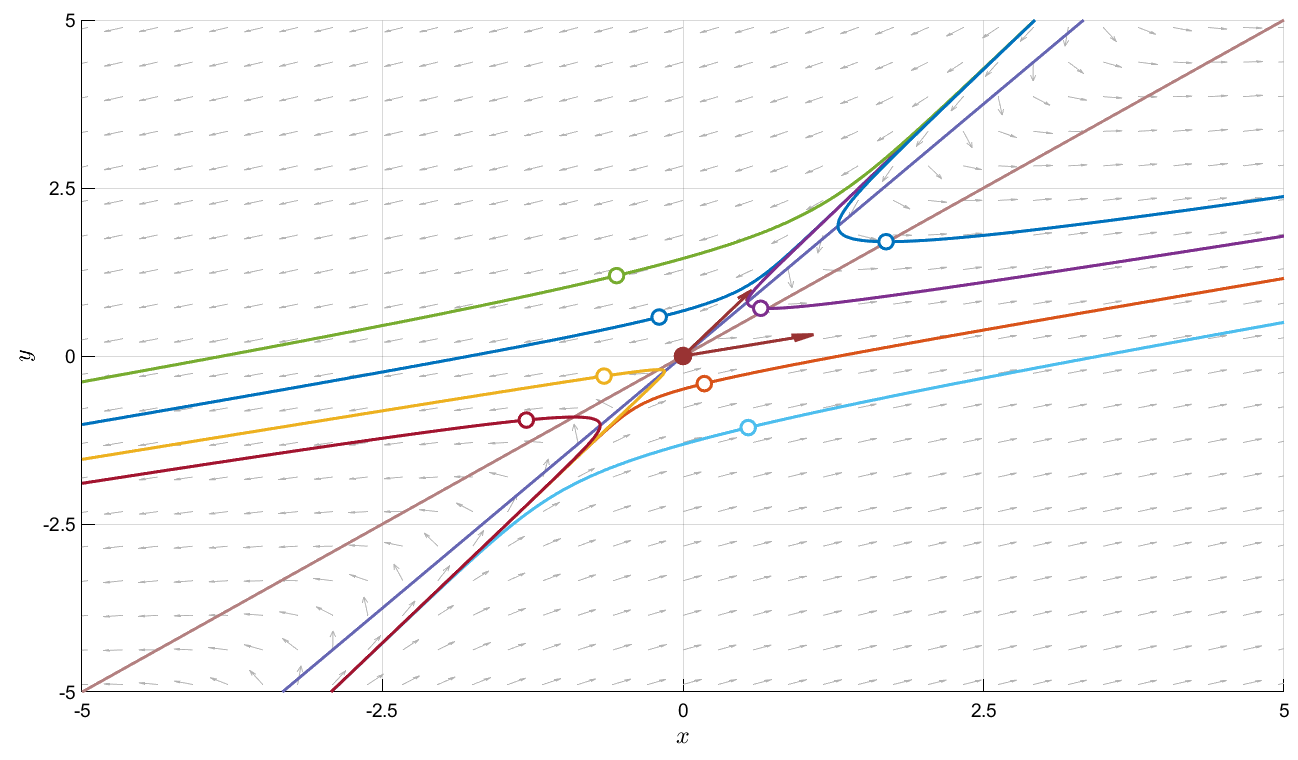
\includegraphics[width=\textwidth]{fig2.3_e.png}
        \caption{$\gamma=2$}
    \end{subfigure}
    \caption{Analysis for potential system 3}
    \label{fig:3}
\end{figure}

\begin{figure}[H]
    \centering
    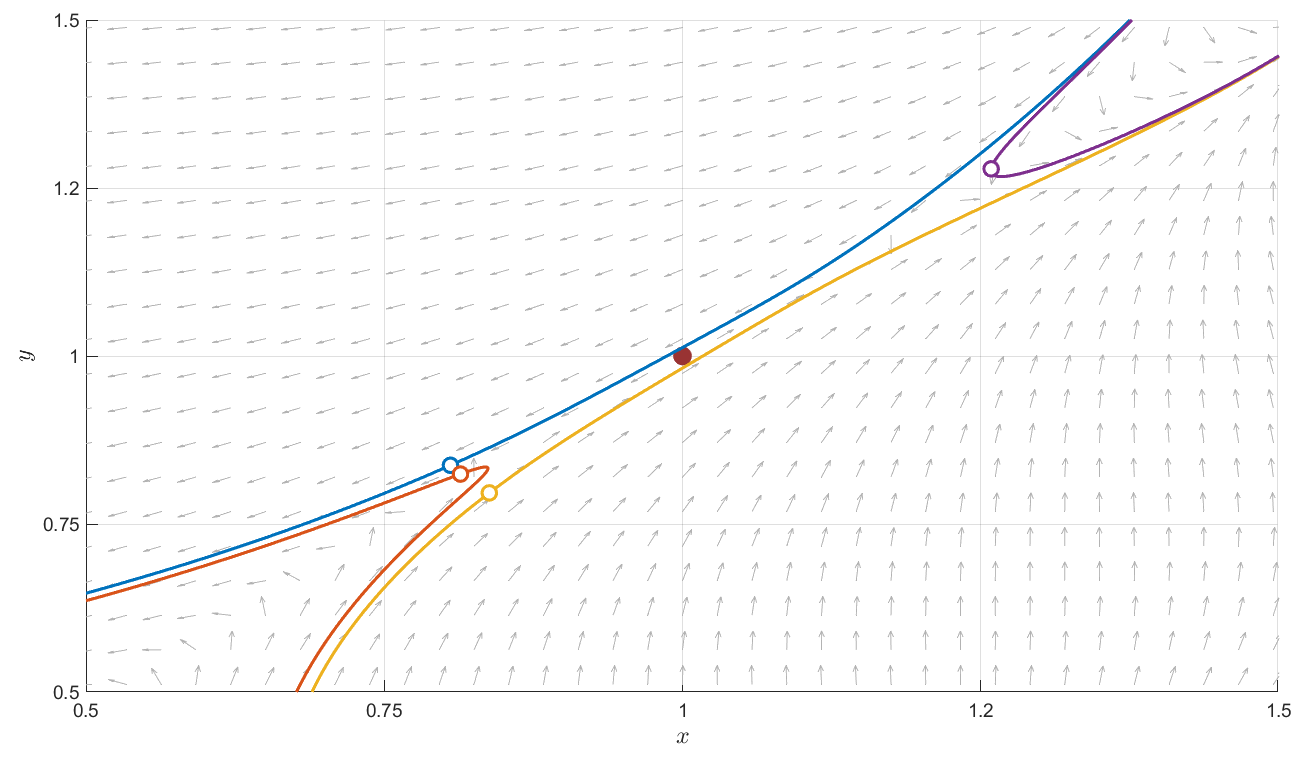
\includegraphics[width=\textwidth]{fig4.2_a.png}
    \caption{$P_3$ analysis}
    \label{fig:4}
\end{figure}

\begin{figure}[H]
    \centering
    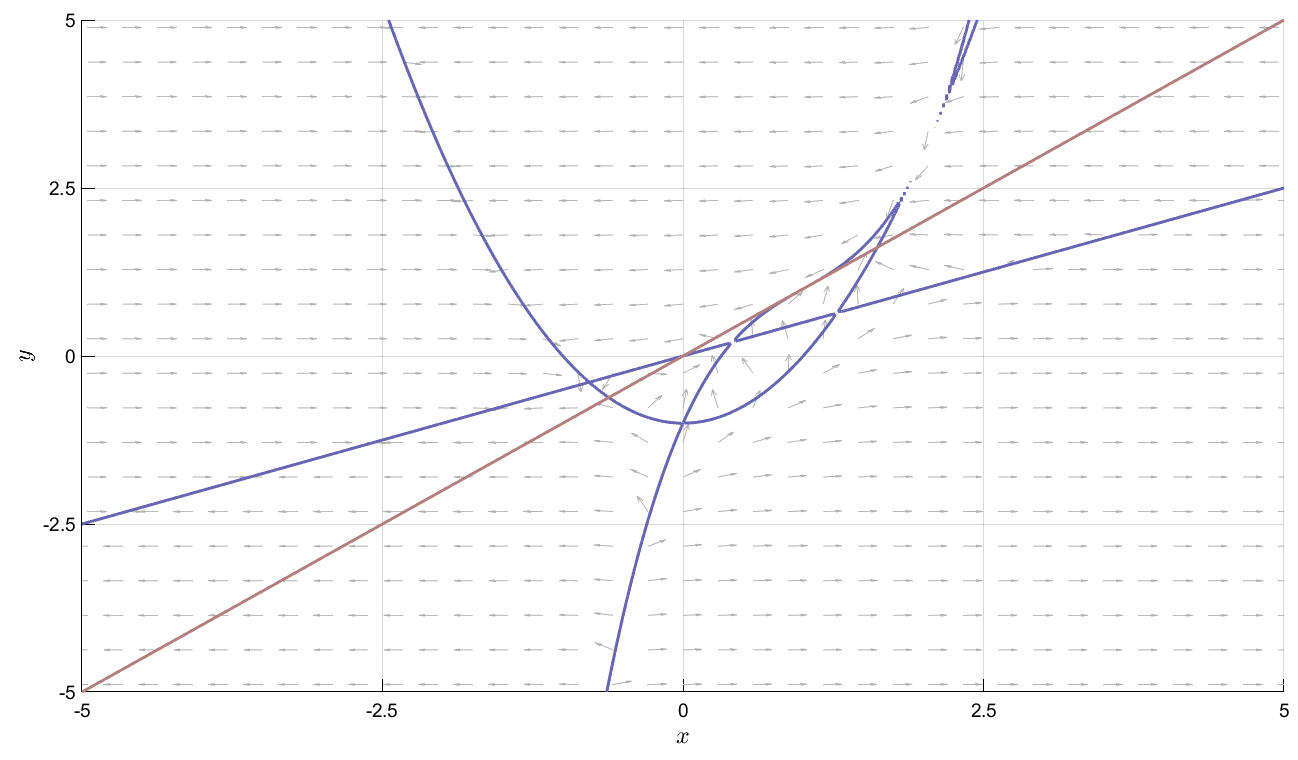
\includegraphics[width=\textwidth]{fig4.4_a.png}
    \caption{Nullclines for the system where $\alpha=-1,\beta=1,\gamma=0$}
    \label{fig:5}
\end{figure}
\begin{figure}[H]
    \centering
    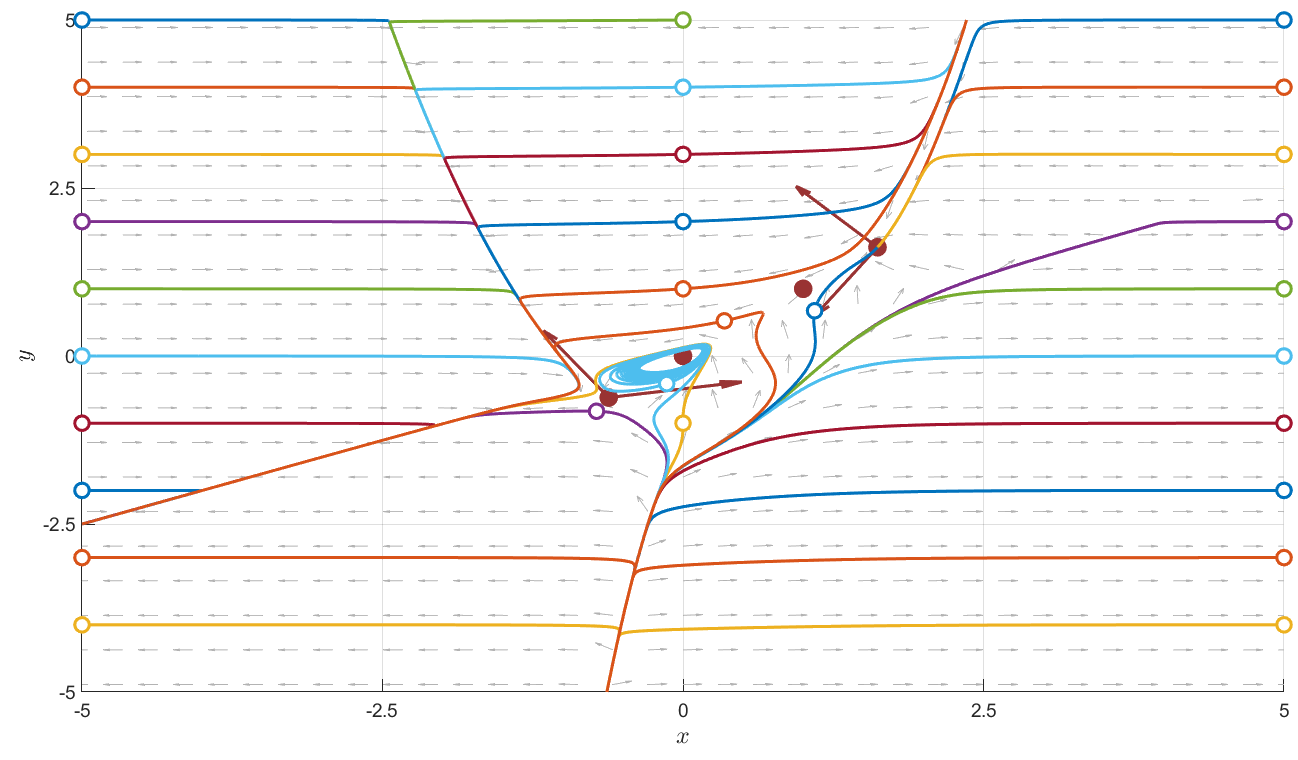
\includegraphics[width=\textwidth]{fig4.4_b.png}
    \caption{Phase portrait for the system where $\alpha=-1,\beta=1,\gamma=0$}
    \label{fig:6}
\end{figure}
\begin{figure}[H]
    \centering
    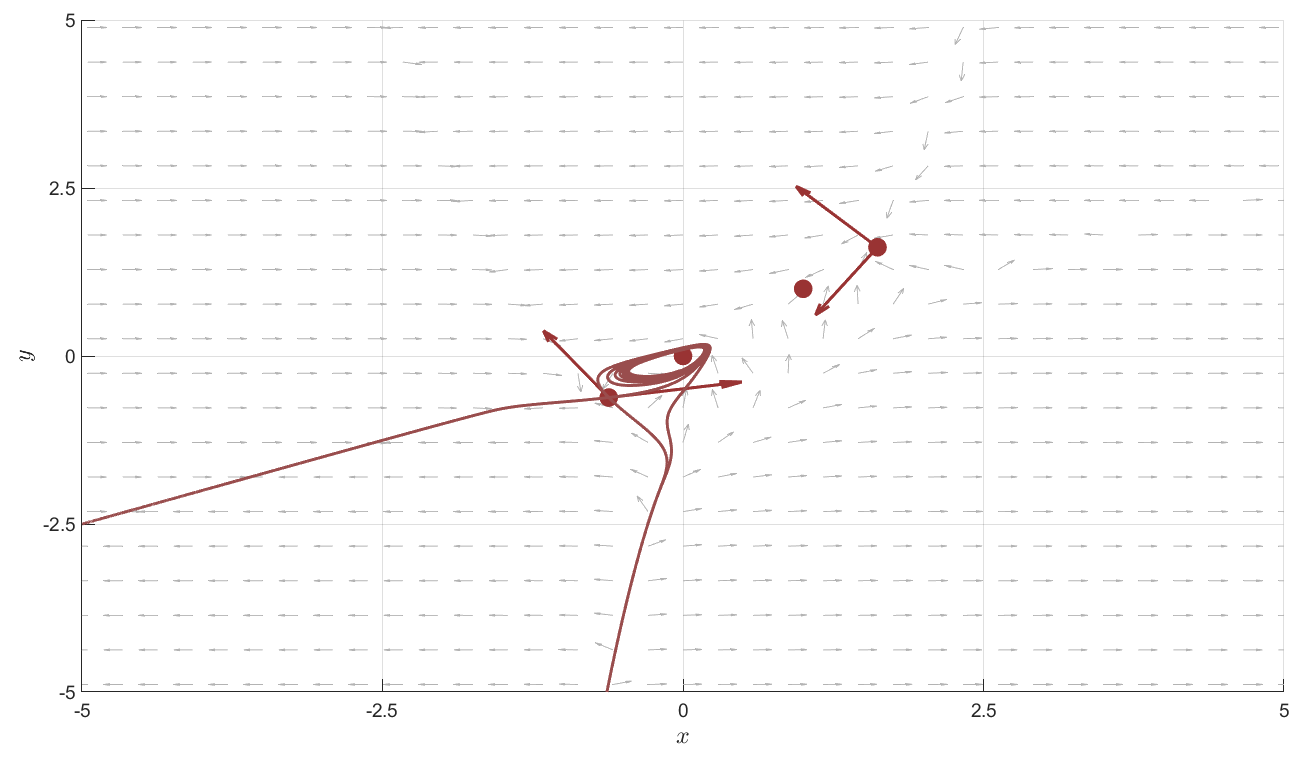
\includegraphics[width=\textwidth]{fig4.4_c.png}
    \caption{Manifolds for the system where $\alpha=-1,\beta=1,\gamma=0$}
    \label{fig:7}
\end{figure}
\begin{figure}[H]
    \centering
    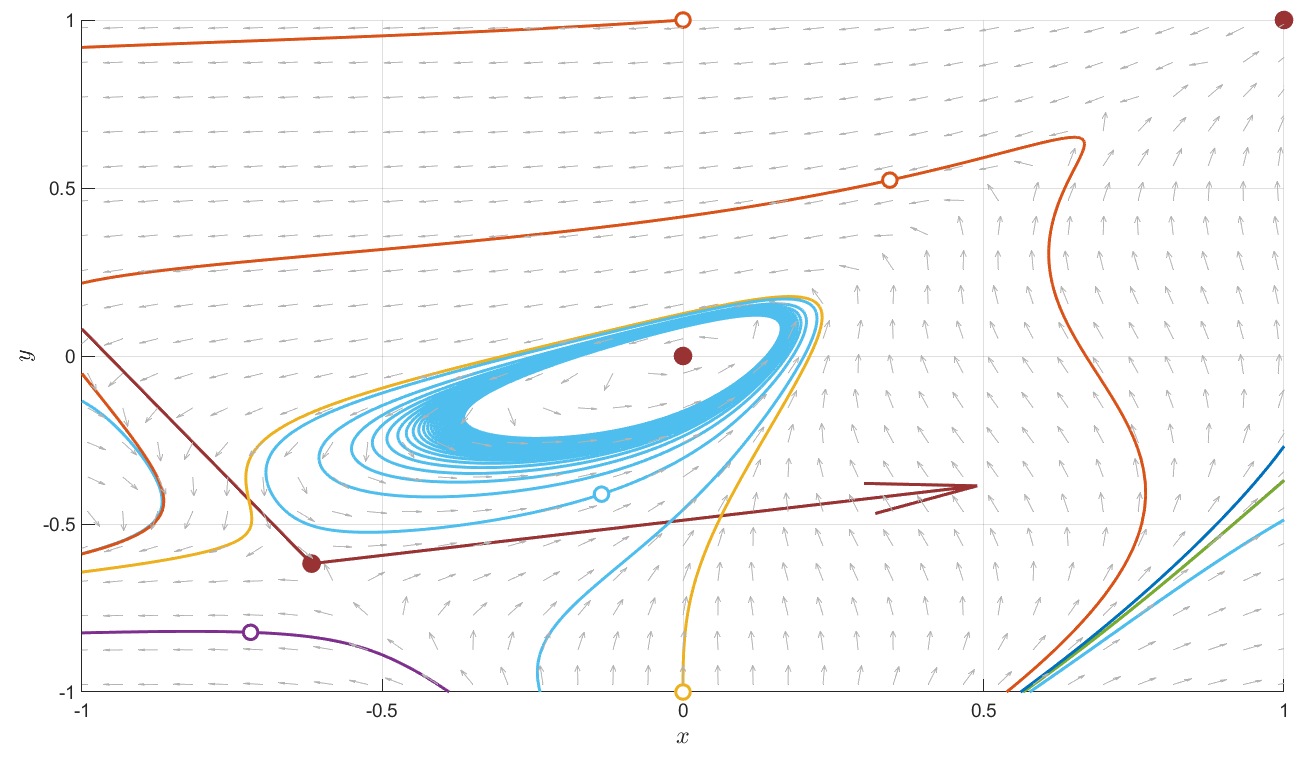
\includegraphics[width=\textwidth]{fig4.4_d.png}
    \caption{Zoomed in image of Figure~\ref{fig:6}}
    \label{fig:8}
\end{figure}

\begin{figure}[H]
    \centering
    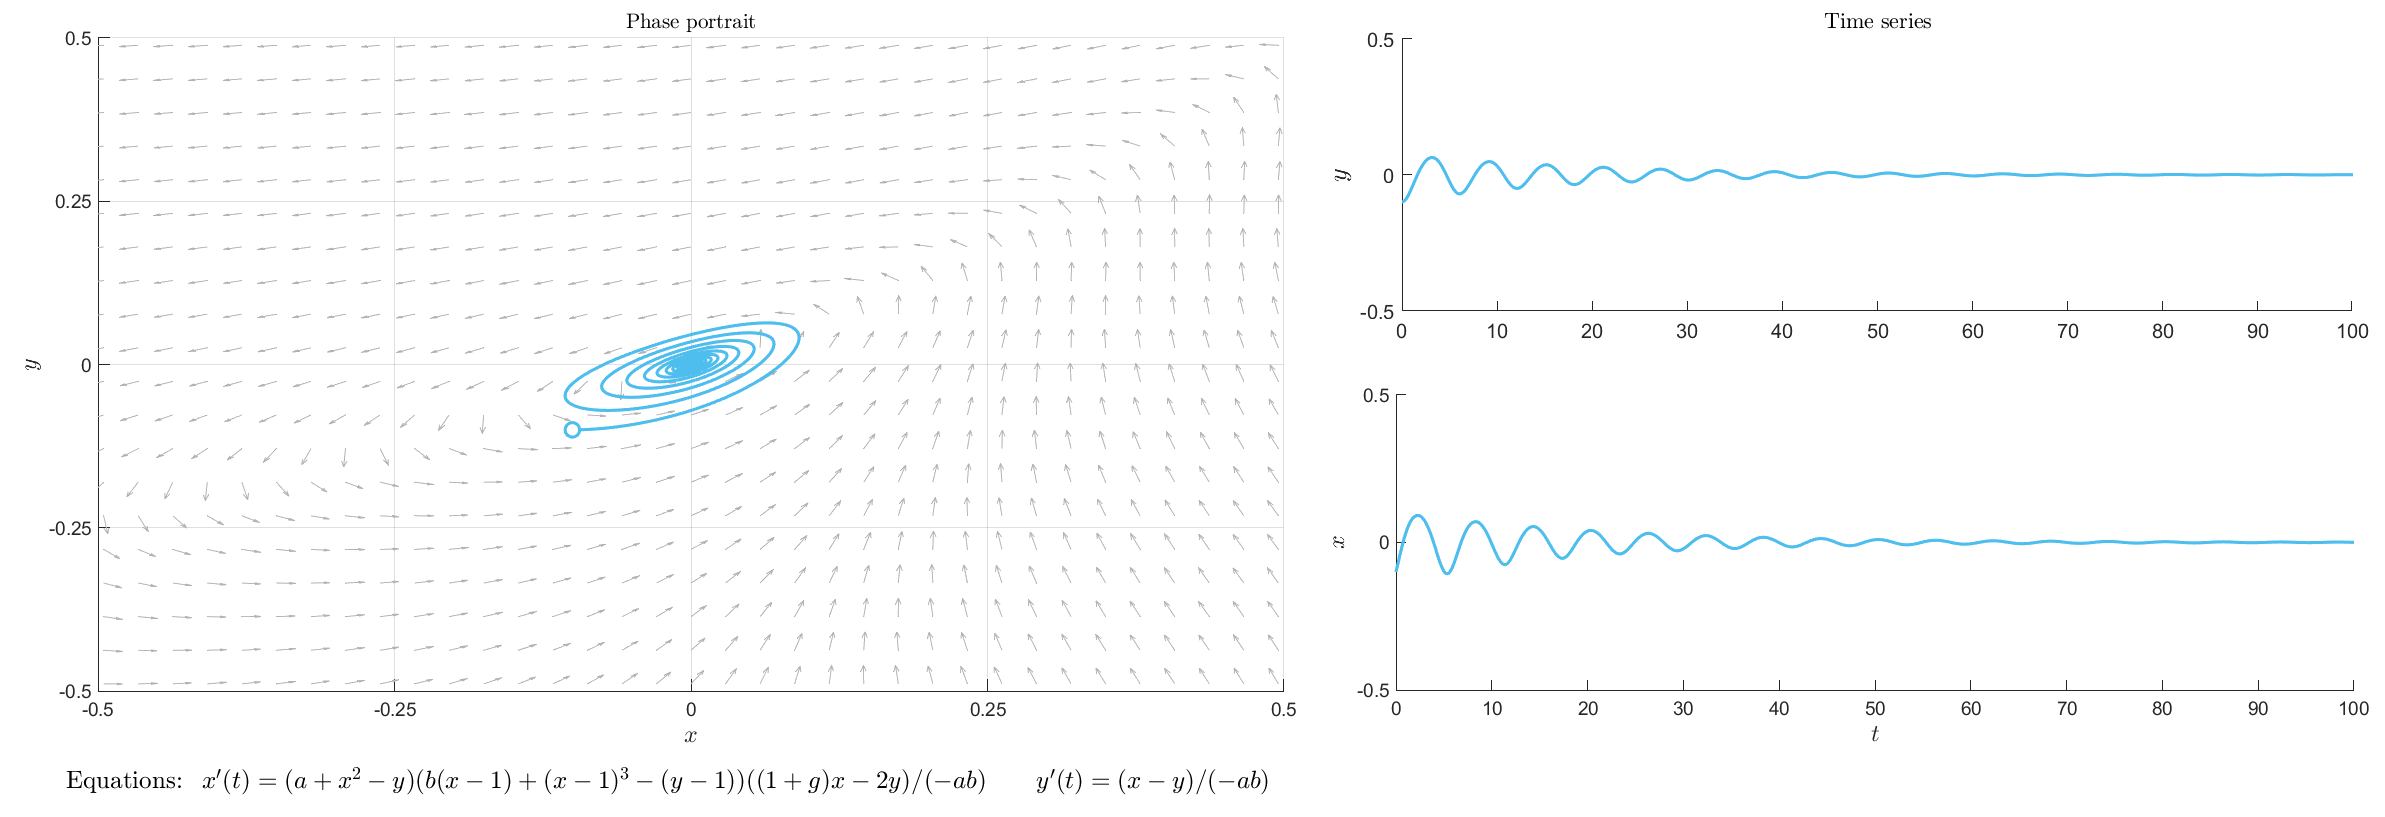
\includegraphics[width=\textwidth]{fig5.1_a.png}
    \caption{Phase portrait of the system where $\alpha=-1, \beta=1, \gamma=-0.1$}
    \label{fig:9}
\end{figure}
\begin{figure}[H]
    \centering
    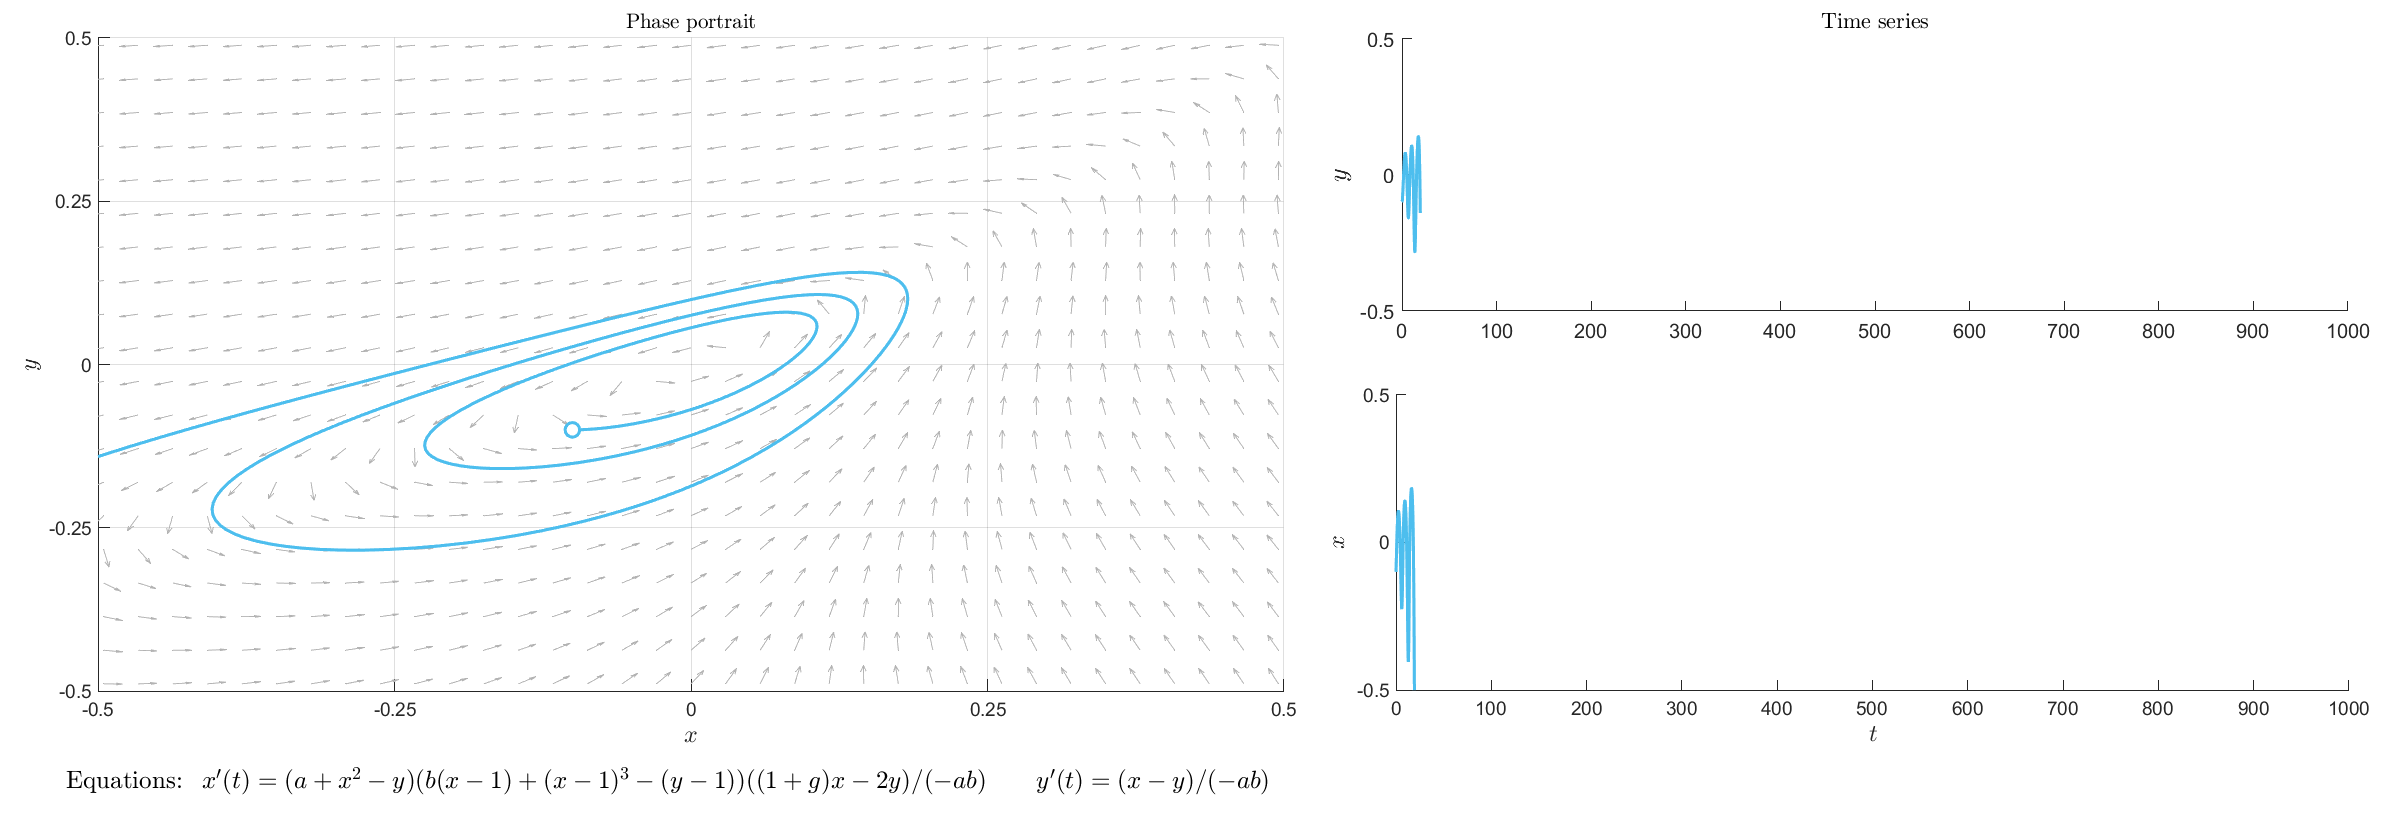
\includegraphics[width=\textwidth]{fig5.1_b.png}
    \caption{Phase portrait of the system where $\alpha=-1, \beta=1, \gamma=0.1$}
    \label{fig:10}
\end{figure}

\begin{figure}[H]
    \centering
    \begin{subfigure}{.49\textwidth}
        \centering
        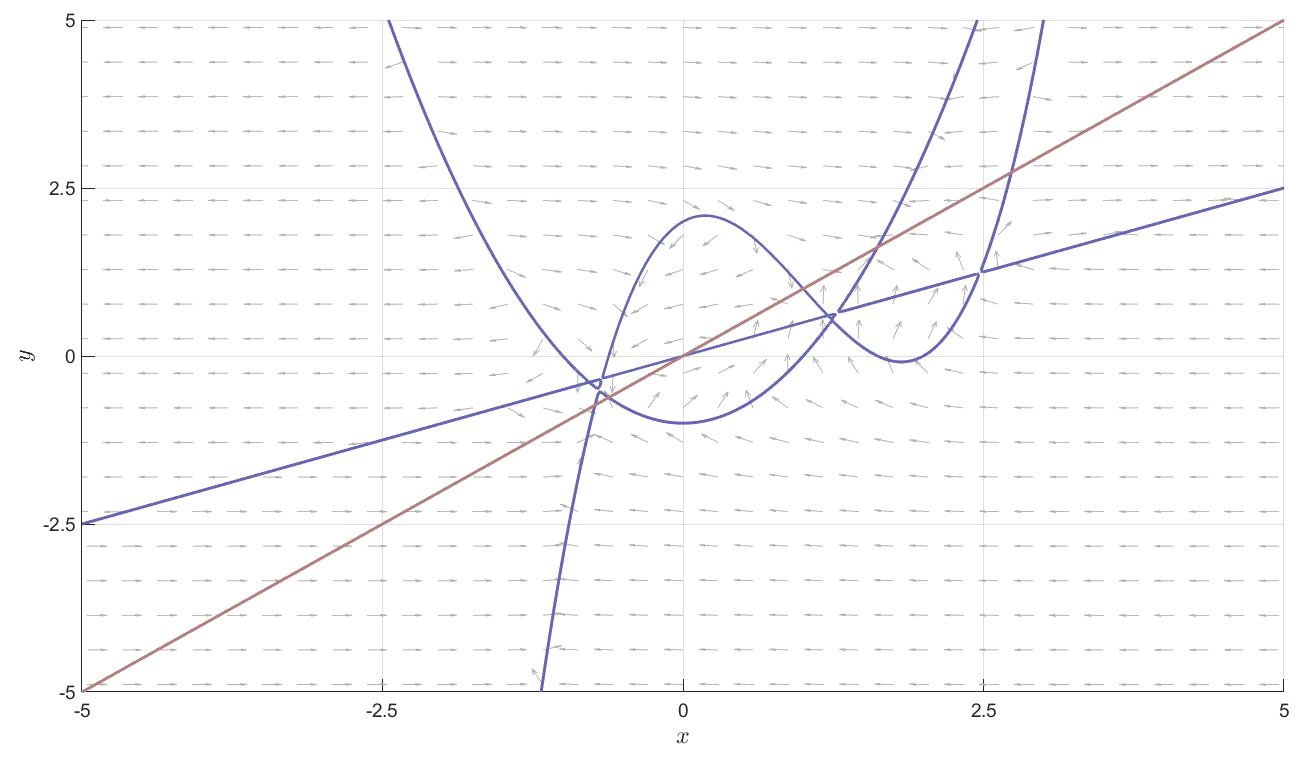
\includegraphics[width=\textwidth]{fig6.1_a.png}
        \caption{Nullclines}
    \end{subfigure}
    \begin{subfigure}{.49\textwidth}
        \centering
        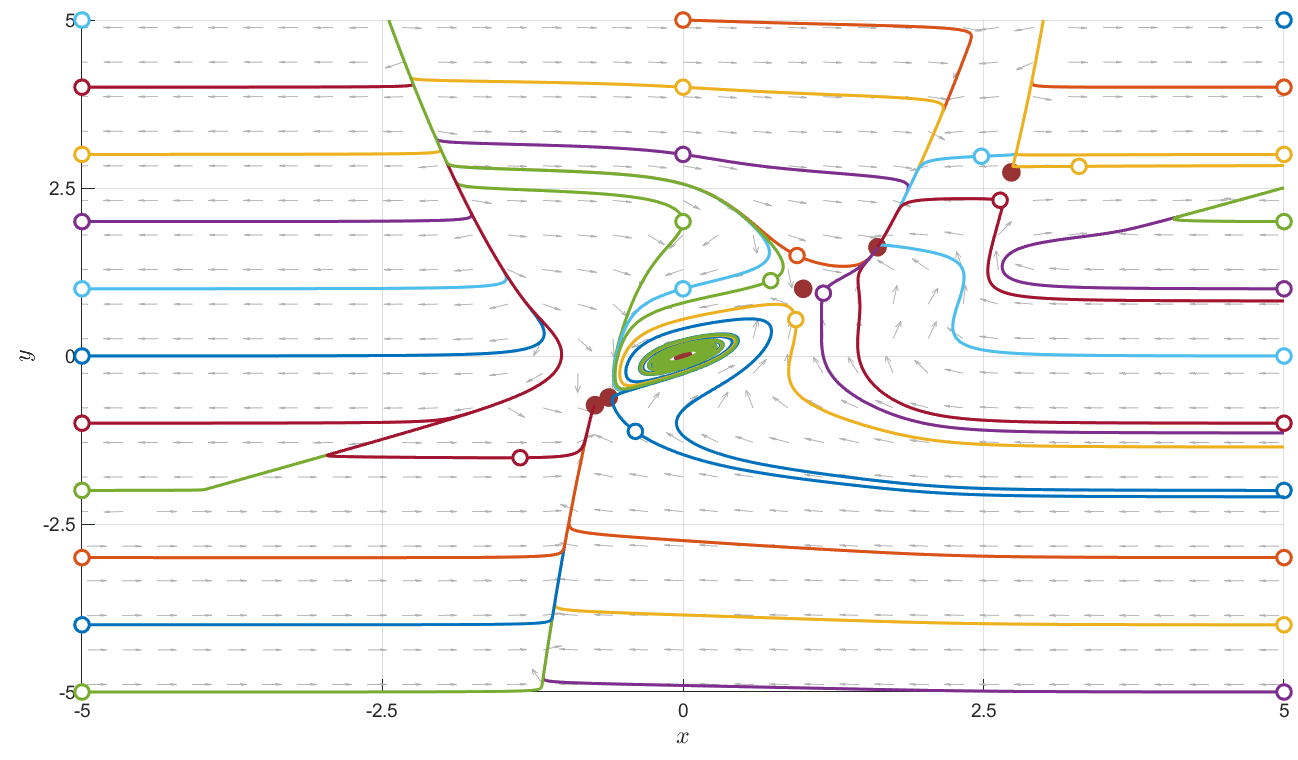
\includegraphics[width=\textwidth]{fig6.1_b.png}
        \caption{Phase Portrait}
    \end{subfigure}
    \caption{Plots for the system where $\alpha=-1, \beta=-2, \gamma=0$}
    \label{fig:11}
\end{figure}
\begin{figure}[H]
    \centering
    \begin{subfigure}{.49\textwidth}
        \centering
        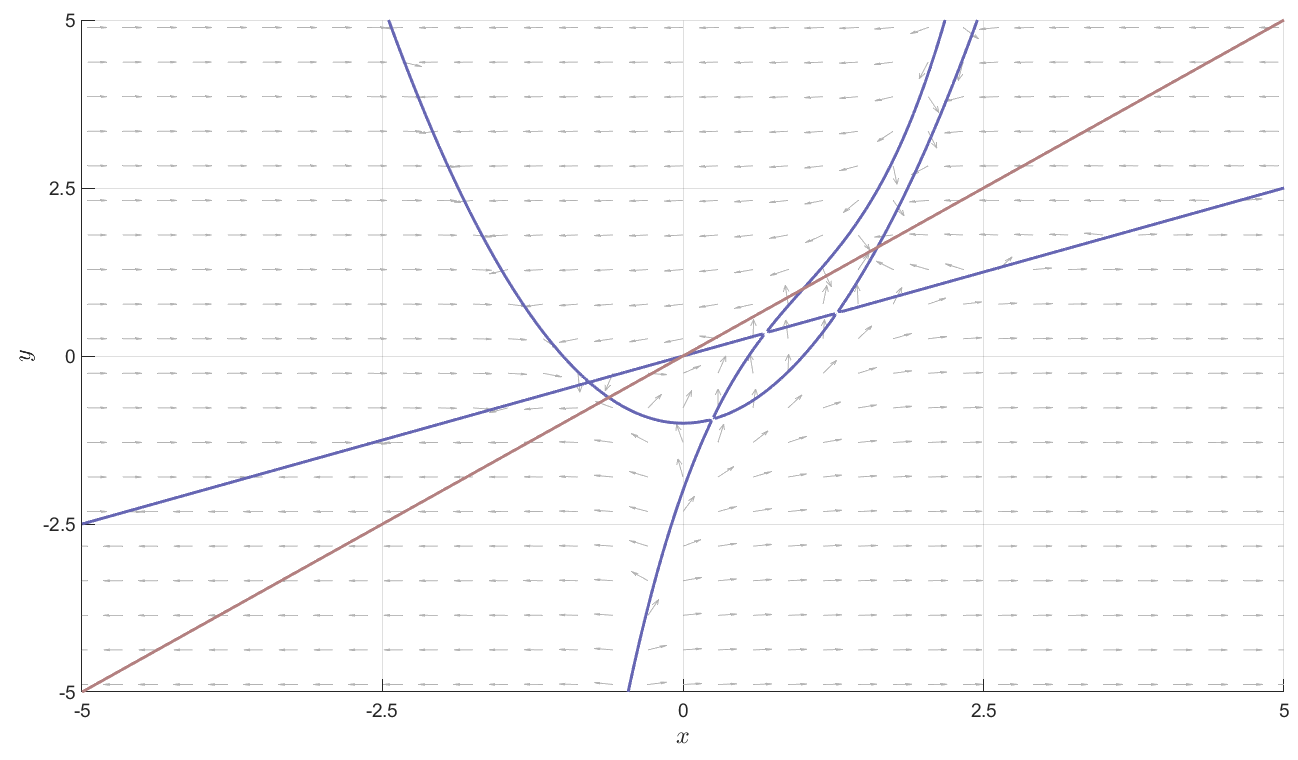
\includegraphics[width=\textwidth]{fig6.1_c.png}
        \caption{Nullclines}
    \end{subfigure}
    \begin{subfigure}{.49\textwidth}
        \centering
        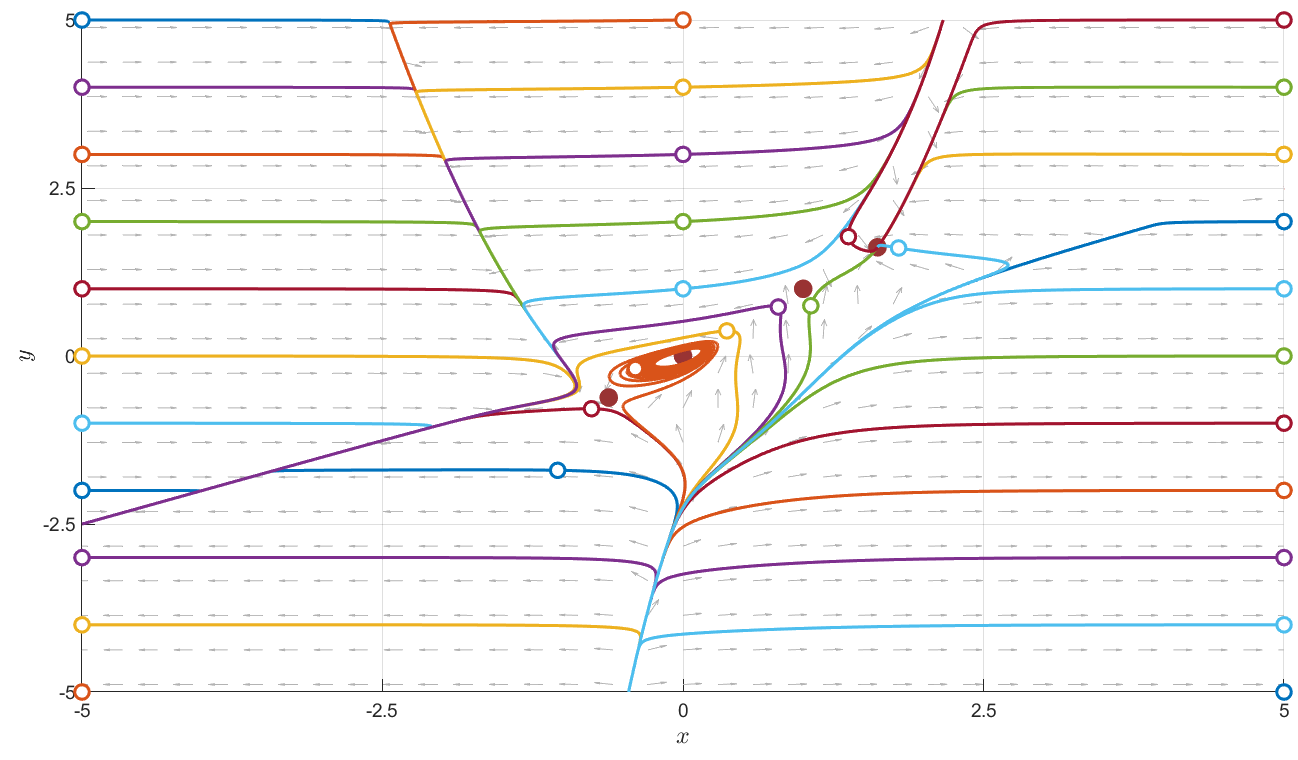
\includegraphics[width=\textwidth]{fig6.1_d.png}
        \caption{Phase Portrait}
    \end{subfigure}
    \caption{Plots for the system where $\alpha=-1, \beta=2, \gamma=0$}
    \label{fig:12}
\end{figure}
